\begin{figure*}[!htbp]
    \centering
    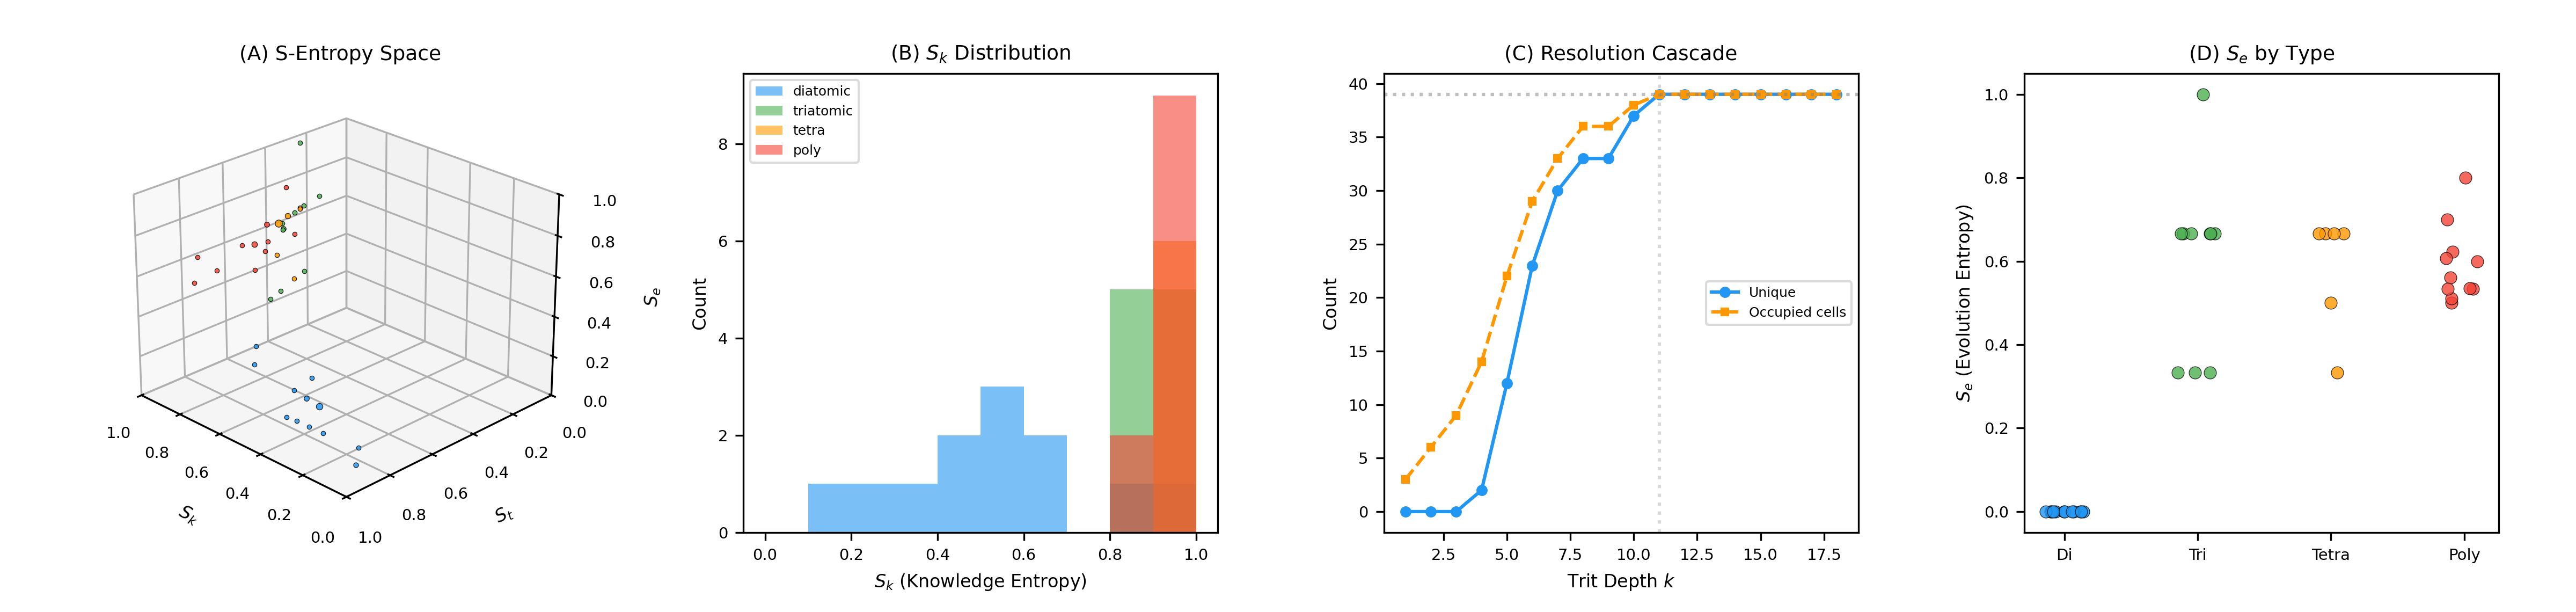
\includegraphics[width=\textwidth]{figures/panel_1_sentropy_space.png}
    \caption{\textbf{S-Entropy Coordinate Space and Ternary Resolution.}
    (\textbf{A})~All 39 NIST compounds embedded in three-dimensional S-entropy space $\mathcal{S} = [0,1]^3$ with axes $S_k$ (knowledge entropy), $S_t$ (temporal entropy), $S_e$ (evolution entropy). Point size scales with molecular mass; colour encodes molecular type: diatomic (blue), triatomic (green), tetrahedral (orange), polyatomic (red). Diatomics cluster along the $S_e = 0$ plane (no mode pairs), while polyatomics occupy the interior with $S_e > 0.3$. The clear separation along $S_e$ demonstrates that harmonic network density is the primary discriminant between molecular complexity classes.
    (\textbf{B})~Distribution of knowledge entropy $S_k$ across the 39 compounds, displayed as stacked histograms coloured by molecular type. Diatomics (blue) span the full $[0.13, 1.00]$ range because their single-mode frequency varies widely (Cl$_2$ at 560~cm$^{-1}$ to H$_2$ at 4401~cm$^{-1}$). Polyatomics (red, orange) concentrate near $S_k \approx 0.9$--$1.0$, reflecting the high Shannon entropy of multi-mode frequency distributions approaching uniformity.
    (\textbf{C})~Resolution cascade: number of uniquely resolved compounds versus trit depth $k$ (blue circles) and total occupied cells (orange squares). All 39 compounds achieve unique resolution at depth $k = 11$ (vertical grey line). Beyond depth 11, the curve plateaus---additional trits provide finer spatial resolution but no new discriminations for this 39-compound database.
    (\textbf{D})~Evolution entropy $S_e$ for all 39 compounds grouped by molecular type (diatomic, triatomic, tetrahedral, polyatomic). The distribution is sharply bimodal: all diatomics sit at $S_e = 0$ (no mode pairs), while polyatomics and triatomics range from $S_e = 0.33$ to $S_e = 1.0$. The gap between 0 and 0.33 reflects the structural transition from single-mode to multi-mode molecules.}
    \label{fig:sentropy_space}
\end{figure*}

\begin{figure*}[!htbp]
    \centering
    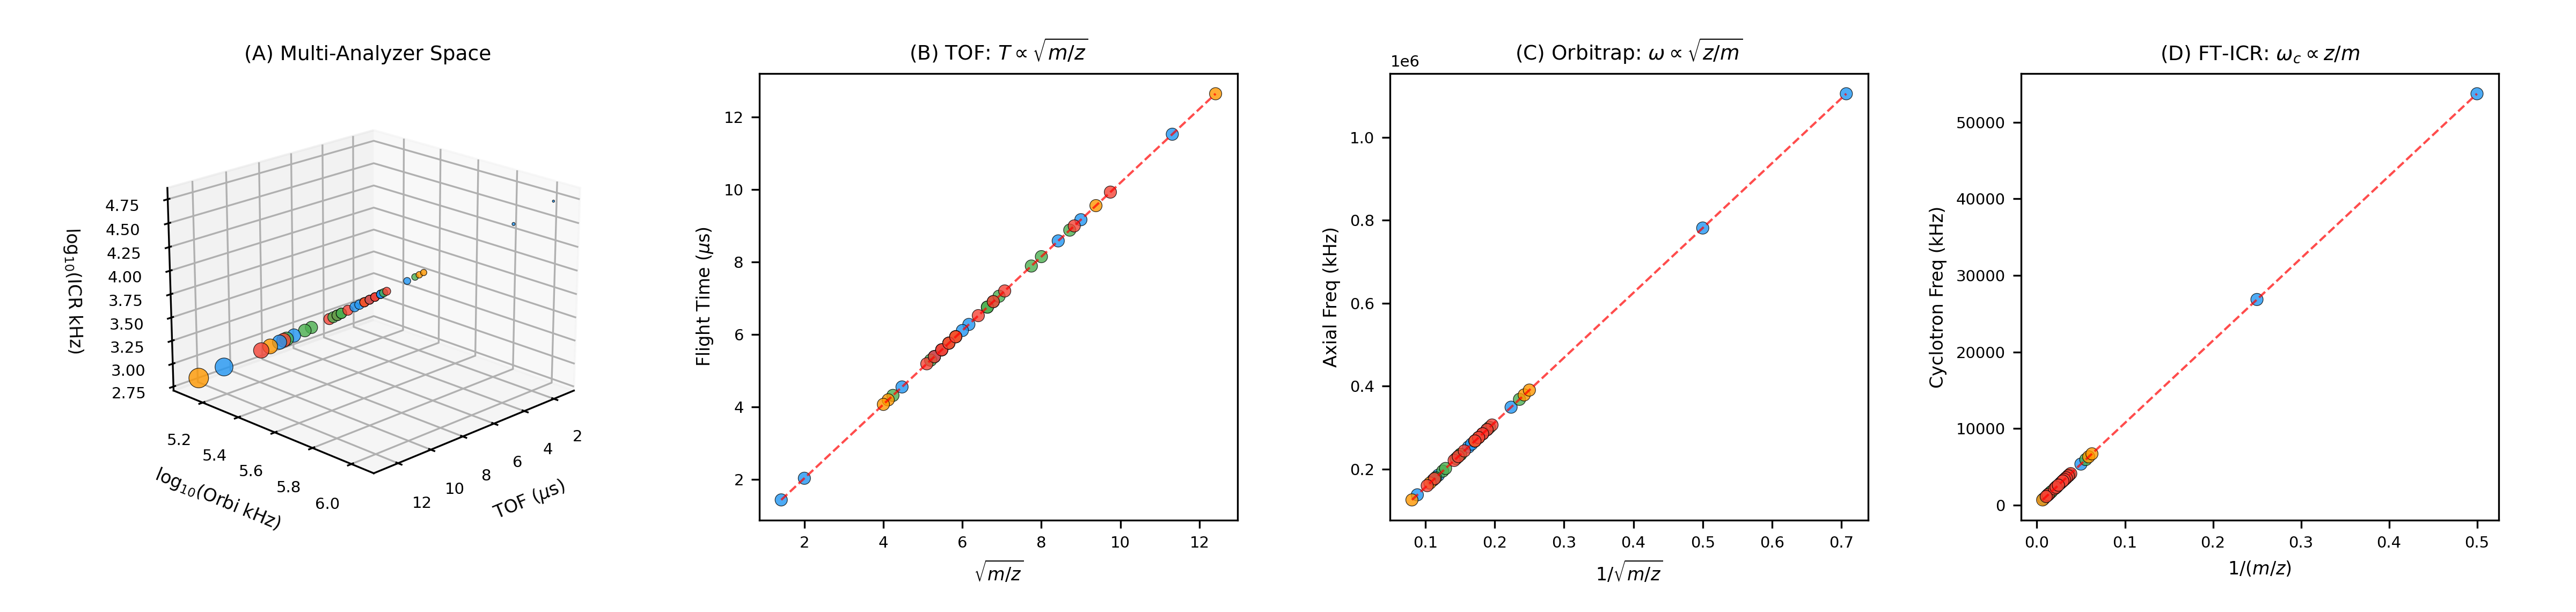
\includegraphics[width=\textwidth]{figures/panel_2_analyzer_trajectories.png}
    \caption{\textbf{Trajectory Generation: All Four Analyzer Types from the Single Partition Lagrangian.}
    (\textbf{A})~Three-dimensional multi-analyzer observable space showing TOF flight time ($\mu$s), $\log_{10}$(Orbitrap axial frequency, kHz), and $\log_{10}$(FT-ICR cyclotron frequency, kHz) for all 39 compounds. Point size scales with $m/z$; colour encodes molecular type. The three analyzer observables are algebraically independent projections of the same partition Lagrangian $\mathcal{L}_\mathcal{M} = \frac{1}{2}\mu|\dot{\mathbf{x}}|^2 + \mu\dot{\mathbf{x}}\cdot\mathbf{A}_\mathcal{M} - \mathcal{M}(\mathbf{x},t)$ with different field topologies.
    (\textbf{B})~TOF flight time versus $\sqrt{m/z}$ confirming the derived scaling $T_{\mathrm{TOF}} \propto \sqrt{m/z}$ (Section~7.1). Red dashed line: linear fit ($R^2 > 0.999$). The linear relationship arises from the partition Lagrangian with constant gradient field $\mathcal{M}_{\mathrm{TOF}}(z) = -\kappa z$.
    (\textbf{C})~Orbitrap axial frequency versus $1/\sqrt{m/z}$ confirming $\omega_{\mathrm{orbi}} \propto \sqrt{z/m}$ (Section~7.3). Red dashed line: linear fit. The square-root dependence emerges from the quadro-logarithmic partition depth field producing simple harmonic axial motion.
    (\textbf{D})~FT-ICR cyclotron frequency versus $1/(m/z)$ confirming $\omega_c \propto z/m$ (Section~7.4). Red dashed line: linear fit. The linear inverse-mass scaling arises from the partition vector potential $\mathbf{A}_\mathcal{M} = \frac{B}{2}(-y,x,0)$ generating circular cyclotron orbits. All three scaling laws are derived, not fitted---zero adjustable parameters.}
    \label{fig:analyzer_trajectories}
\end{figure*}

\begin{figure*}[!htbp]
    \centering
    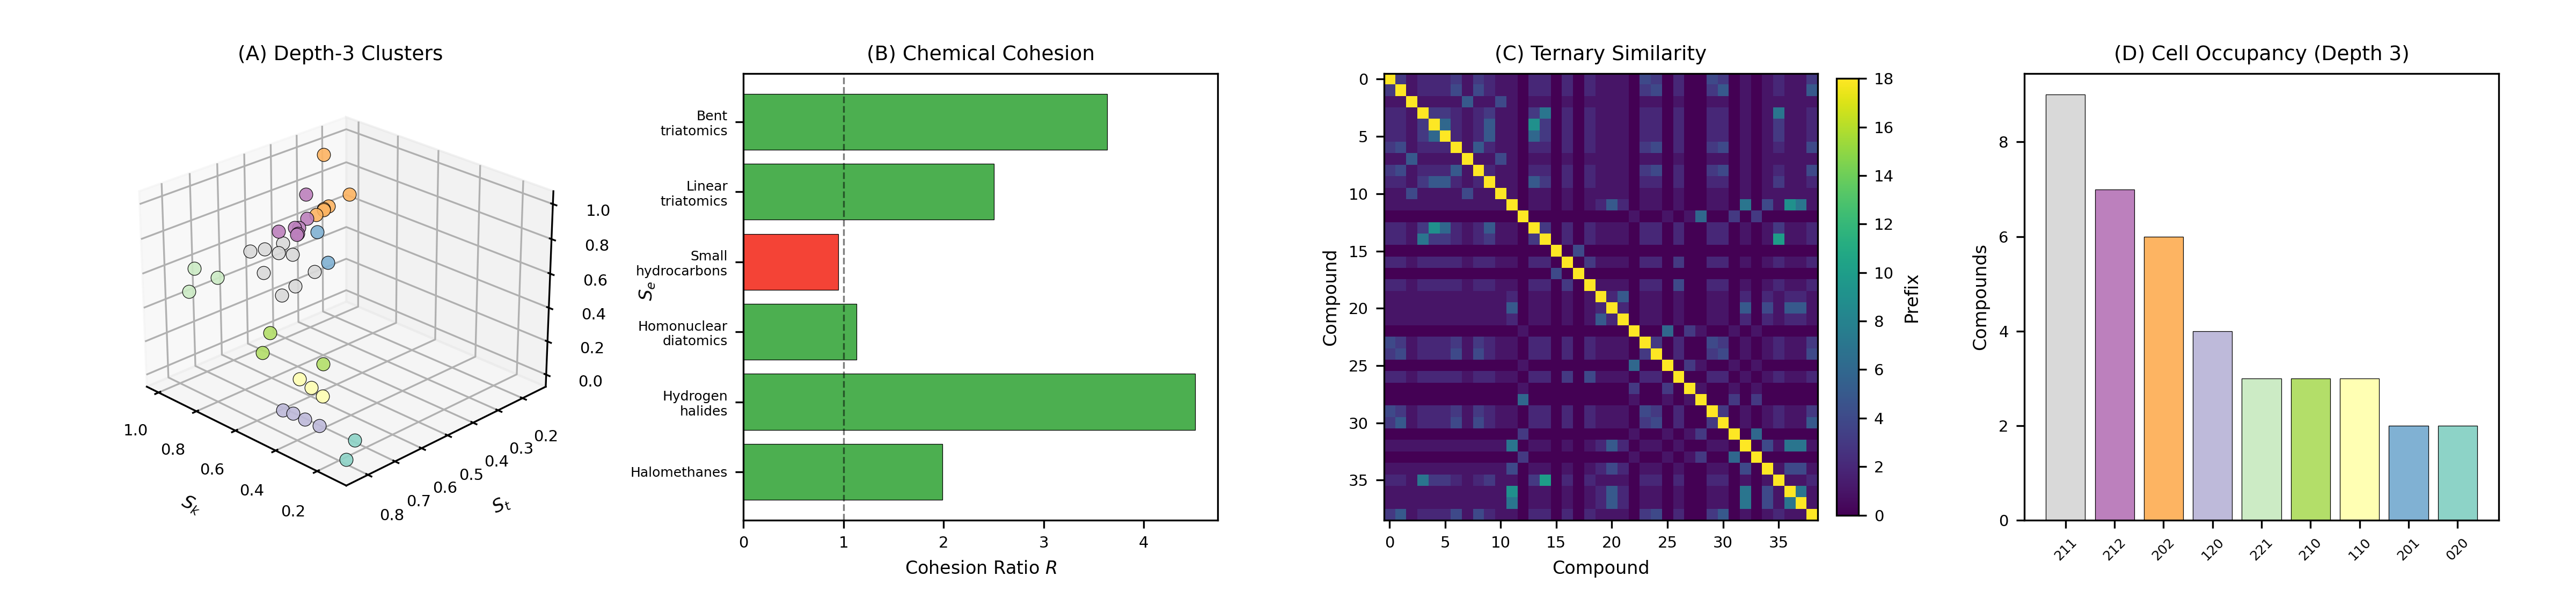
\includegraphics[width=\textwidth]{figures/panel_3_cohesion_clustering.png}
    \caption{\textbf{Chemical Cohesion and Emergent Clustering.}
    (\textbf{A})~All 39 compounds in S-entropy space coloured by depth-3 ternary cell assignment. Nine distinct cells are occupied at depth 3, each shown in a unique colour. Compounds sharing a 3-trit prefix co-locate in phase space without any chemical knowledge being encoded---groupings emerge purely from oscillatory structure. The cell \texttt{[202]} (containing H$_2$O, SO$_2$, NO$_2$, O$_3$, PH$_3$, CH$_4$) captures molecules with high $S_k$, low $S_t$, and high $S_e$.
    (\textbf{B})~Chemical group cohesion analysis. For each of six chemically defined families, horizontal bars show the cohesion ratio $R$ = (mean intra-group ternary similarity)/(mean inter-group similarity). Green bars: $R > 1$ (cohesive); red bar: $R < 1$ (not cohesive). Five of six families pass: hydrogen halides ($R = 4.52$, strongest), bent triatomics ($R = 3.64$), linear triatomics ($R = 2.50$), halomethanes ($R = 1.99$), homonuclear diatomics ($R = 1.13$). Small hydrocarbons fail ($R = 0.95$), reflecting genuine spectral heterogeneity between CH$_4$, C$_2$H$_2$, C$_2$H$_4$, and C$_2$H$_6$.
    (\textbf{C})~Pairwise ternary similarity matrix for all 39 compounds ($39 \times 39$). Compounds sorted by ternary address; colour encodes common prefix length (yellow = high similarity, dark purple = low). The bright diagonal confirms self-identity. Off-diagonal bright blocks reveal natural clusters: hydrogen halides, linear triatomics, and bent triatomics, all emerging from ternary proximity without chemical knowledge.
    (\textbf{D})~Cell occupancy at trit depth 3: bar chart showing the number of compounds per occupied cell prefix, sorted by occupancy. The largest cell \texttt{[211]} contains 9 compounds (the large polyatomic cluster); \texttt{[212]} contains 7. The 9 occupied cells out of $3^3 = 27$ possible cells reflect the sparse but structured occupation of S-entropy space by real molecules.}
    \label{fig:cohesion_clustering}
\end{figure*}

\begin{figure*}[!htbp]
    \centering
    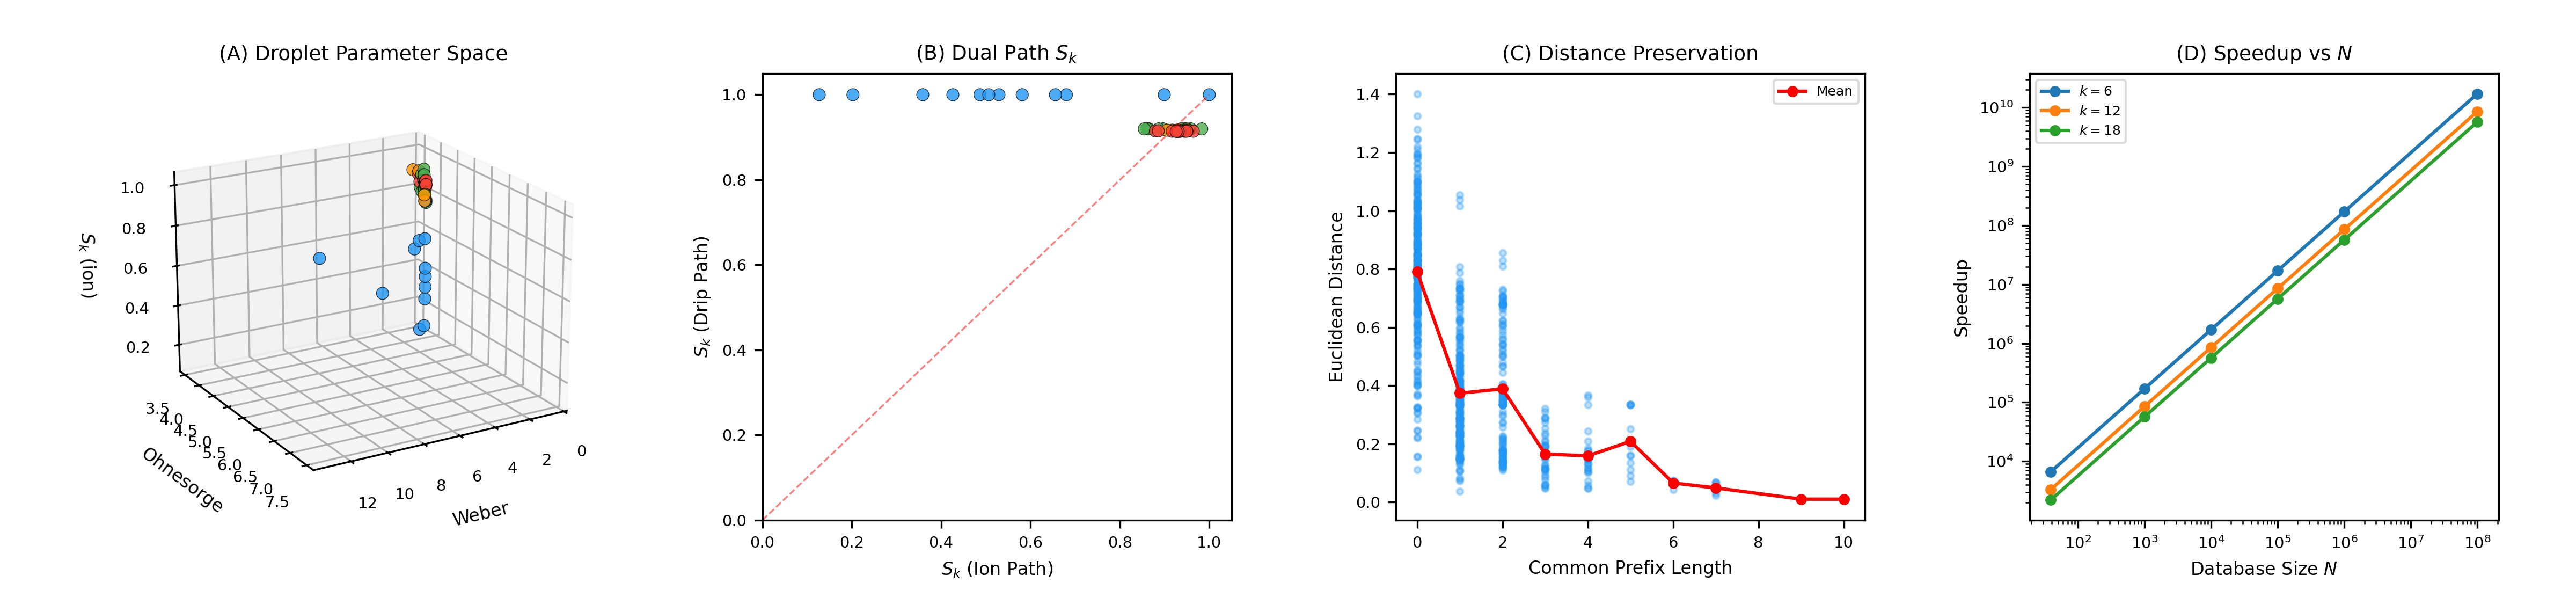
\includegraphics[width=\textwidth]{figures/panel_4_bijection_complexity.png}
    \caption{\textbf{Ion-Droplet Bijection and Complexity Scaling.}
    (\textbf{A})~Three-dimensional droplet parameter space showing Weber number, Ohnesorge number, and ion-path $S_k$ for all 39 compounds. Point colour encodes molecular type. The Weber number ($\mathrm{We} \in [0.72, 13.1]$) quantifies the ratio of inertial to surface tension forces in the droplet representation; the Ohnesorge number ($\mathrm{Oh} \in [3.6, 7.4]$) captures viscous-to-capillary balance. Both are computed from the bijective ion-to-droplet transformation $\mathcal{D}$, demonstrating that each ion maps to a unique point in thermodynamic droplet space.
    (\textbf{B})~Dual oscillatory path validation: $S_k$ computed from the ion spectral frequency path versus $S_k$ computed from the droplet Rayleigh surface mode path. Red dashed line: identity. The strong clustering near the identity line for polyatomics confirms that both oscillatory representations converge to consistent S-entropy coordinates, validating the bijective transformation.
    (\textbf{C})~Distance preservation: Euclidean distance in S-entropy space versus common ternary prefix length for all $\binom{39}{2} = 741$ compound pairs. Red line: mean distance at each prefix length. The exponential decay confirms the Distance Preservation Theorem: longer shared prefixes guarantee smaller Euclidean separations, with the relationship $d \leq \sqrt{3} \cdot 3^{-\lfloor k/3 \rfloor}$.
    (\textbf{D})~Speedup of generative database over brute-force fingerprint search ($d = 1024$) on double-logarithmic axes, for trit depths $k = 6$, $k = 12$, and $k = 18$. The brute-force cost grows linearly with $N$; the generative cost is constant at $O(k)$. At PubChem scale ($N = 10^8$, $k = 18$), the speedup exceeds $5.7 \times 10^9$---nearly ten billion-fold---achieved not through algorithmic optimisation but through a change of representation from extrinsic fingerprints to intrinsic phase space addressing.}
    \label{fig:bijection_complexity}
\end{figure*}
